%Created with command:
%"/home/josh/Teaching/trunk/Utilities/makeexam" "Exam 1" "Please complete each problem.  Show all of your work even if you cannot obtain the correct answer.  You may use only a single sheet of letter sized paper for assistance." "../NumberSystems/Assessments/convert_binary_decimal_ex.tex" "../NumberSystems/Assessments/convert_hex_oct_bin_ex.tex" "../NumberSystems/Assessments/convert_hex_decimal_ex.tex" "../NumberSystems/Assessments/twos_complement_ex.tex" "../NumberSystems/Assessments/twos_complement_arithmetic_ex.tex" "../CMOSCircuits/Assessments/cmos_OR_gate_design.tex" "../CMOSCircuits/Assessments/dc_noise_margin_ex.tex" "../CombinationalCircuits/Assessments/simplify_logic_functions_ex.tex" "../CombinationalCircuits/Assessments/kmaps_ex.tex" "../CombinationalCircuits/Assessments/circuit_design_ex.tex"
\documentclass{article}
\usepackage[T1]{fontenc}
\usepackage{arev}
\usepackage{longtable}
\usepackage[hmargin=2cm,vmargin=2cm]{geometry}
\usepackage{graphicx}
\setlength{\parindent}{0pt}
\title{Exam 1}
\date{}
\begin{document}
\maketitle
Please complete each problem.  Show all of your work, even if you cannot obtain the correct answer.  You may use only a single sheet of letter sized paper for assistance. (40 points total)
\begin{longtable}[l]{rp{17cm}}
%file: ../NumberSystems/Assessments/convert_binary_decimal_ex.tex
1.&\begin{minipage}[t]{\linewidth}(2 pt) Convert the following binary numbers to decimal. \\
\\
(a) $11100001_2$ \\
(b) $0001.101_2$ \\

Solution: \\
\\
(a) $11100001_2 = 1 \cdot 2^7 + 1 \cdot 2^6 + 1 \cdot 2^5 + 1 \cdot 2^0 = 128 + 64 + 32 + 1 = 225$ \\
(b) $0001.101_2 = 1 \cdot 2^0 + 1 \cdot 2^{-1} + 1 \cdot 2^{-3} = 1 + 0.5 + 0.125 = 1.625$ \\
\end{minipage}\\
\medskip
%file: ../NumberSystems/Assessments/convert_hex_oct_bin_ex.tex
2.&\begin{minipage}[t]{\linewidth}(4 pt) Perform the following number system conversions. \\
\\
(a) $00101011_2 = ?_{16}$ \\
(b) $163_{16} = ?_8$ \\

Solution: \\
\\
(a) $00101011_2 = 0010_2 1011_2 = 2\textrm{B}_{16}$ \\
(b) $163_{16} = 0001_2 0110_2 0011_2 = 000_2 101_2 100_2 011_2 = 543_8$ \\
\\
\end{minipage}\\
\medskip
%file: ../NumberSystems/Assessments/convert_hex_decimal_ex.tex
3.&\begin{minipage}[t]{\linewidth}(2 pt) Convert the following hexadecimal number to decimal. \\
\\
$19\textrm{CA}_{16}$ \\

Solution: \\
\\
$19\textrm{CA}_{16} = 1 \cdot 16^3 + 9 \cdot 16^2 + 12 \cdot 16^1 + 10 \cdot 16^0 = 1 \cdot 4096 + 9 \cdot 256 + 12 \cdot 16 + 10 \cdot 1 = 6602$ \\
\\
\end{minipage}\\
\medskip
%file: ../NumberSystems/Assessments/twos_complement_ex.tex
4.&\begin{minipage}[t]{\linewidth}(2 pt) Find the eight bit two's complement representation of each of the following numbers. \\
\\
(a) $-10$\\
(b) $-36$

Solution: \\
\\
(a)\\
\begin{tabular}{rl}
  $10 =$ & $00001010_2$\\
         & $\Downarrow \textrm{complement}$\\
         & $11110101_2$\\
     $+$ & $00000001_2$\\
         & $11110110_2$\\
         & $= 1 \cdot -128 + 1 \cdot 64 + 1 \cdot 32 + 1 \cdot 16 + 1 \cdot 4 + 1 \cdot 2= -10$
\end{tabular}\\
\\
(b)\\
\begin{tabular}{rl}
  $36 =$ & $00100100_2$\\
         & $\Downarrow \textrm{complement}$\\
         & $11011011_2$\\
     $+$ & $00000001_2$\\
         & $11011100_2$\\
         & $= 1 \cdot -128 + 1 \cdot 64 + 1 \cdot 16 + 1 \cdot 8 + 1 \cdot 4 = -36$
\end{tabular}\\
\end{minipage}\\
\medskip
%file: ../NumberSystems/Assessments/twos_complement_arithmetic_ex.tex
5.&\begin{minipage}[t]{\linewidth}(6 pt) Perform the following binary arithmetic using the four bit two's complement representation, showing all carries.  For each case, determine if overflow occurs. If it does, state why it occurs.
\\
\\
(a) $4 - 3$\\
(b) $5 + -1$\\

%vspace 6cm
Solution: \\
\\
(a)\\
$4 = 0100_2$\\
$3 = 0011_2$\\
Note that $-3$ complement is $1100_2$ and remember to use $c_{in}=1$.\\
\\
\begin{tabular}{cccccc}
  C & 1 & 1 & 0 & 0 & 1 \\
    &   & 0 & 1 & 0 & 0 \\
    & + & 1 & 1 & 0 & 0 \\
  \hline
    &   & 0 & 0 & 0 & 1 \\
\end{tabular} \\
\\
Overflow does not occur.\\
\\
(b)\\
$5 = 0101_2$\\
$-1 = 1111_2$\\
\\
\begin{tabular}{cccccc}
  C & 1 & 1 & 1 & 1 & 0 \\
    &   & 0 & 1 & 0 & 1 \\
    & + & 1 & 1 & 1 & 1 \\
  \hline
    &   & 0 & 1 & 0 & 0 \\
\end{tabular} \\
\\
Overflow does not occur.\\
\end{minipage}\\
\medskip
%file: ../CMOSCircuits/Assessments/cmos_OR_gate_design.tex
6.&\begin{minipage}[t]{\linewidth}(4 pt) Write the function table and draw the circuit diagram for a two input CMOS OR gate.  Note that this gate should use six transistors.\\ \\

Solution: \\ \\
\begin{tabular}{ccccccccc}
  \textbf{A} & \textbf{B} & \textbf{Q1} & \textbf{Q2} & \textbf{Q3} & \textbf{Q4} & \textbf{Q5} & \textbf{Q6} & \textbf{Z} \\
  \hline
  L & L & off & on & off & on & on & off & L\\
  L & H & off & on & on & off & off & on & H\\
  H & L & on & off & off & on & off & on & H\\
  H & H & on & off & on & off & off & on & H\\
\end{tabular}
\medskip
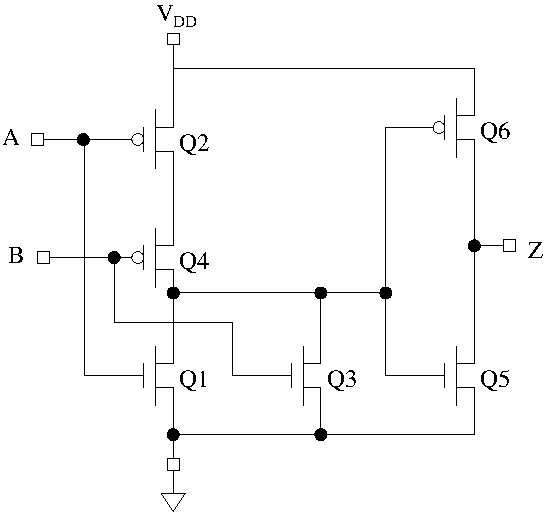
\includegraphics{../CMOSCircuits/Assessments/CMOSORGate}
\end{minipage}\\
\medskip
%file: ../CMOSCircuits/Assessments/dc_noise_margin_ex.tex
7.&\begin{minipage}[t]{\linewidth}(2 pt) Given the following information from a data sheet, compute the HIGH and LOW state DC noise margins.\\ \\
$\textrm{V}_{\textrm{OHmin}} = 3.7 \textrm{V}$\\
$\textrm{V}_{\textrm{IHmin}} = 2.8 \textrm{V}$\\
$\textrm{V}_{\textrm{ILmax}} = 1.9 \textrm{V}$\\
$\textrm{V}_{\textrm{OLmax}} = 0.4 \textrm{V}$\\

Solution: \\ \\
HIGH state: $\textrm{V}_{\textrm{OHmin}} - \textrm{V}_{\textrm{IHmin}} = 0.9 \textrm{V}$\\
LOW state: $\textrm{V}_{\textrm{ILmax}} - \textrm{V}_{\textrm{OLmax}} = 1.5 \textrm{V}$\\
\end{minipage}\\
\medskip
%file: ../CombinationalCircuits/Assessments/simplify_logic_functions_ex.tex
8.&\begin{minipage}[t]{\linewidth}(6 pt) Using the theorems of switching algebra, simplify the following logic functions to a sum of of products representation.\\ \\
(a) $F=X' \cdot Y \cdot Z + Y \cdot X + X \cdot Y \cdot Z + Z \cdot X \cdot Y$ \\
(b) $F=Z \cdot (X' + Y') + X \cdot Y \cdot Z$ \\

Solution: \\ \\
(a)\\
\begin{tabular}{rll}
  $F$ & $=X' \cdot Y \cdot Z + Y \cdot X + X \cdot Y \cdot Z + Z \cdot X \cdot Y$ &\\
  $F$ & $=Y \cdot Z + Y \cdot X + Z \cdot X \cdot Y$ & (T10)\\
      & $=Y \cdot Z + Y \cdot X$ & (T9)\\
\end{tabular}\\ \\
(b)\\
Note: $X' + Y' = (X \cdot Y)'$ by (T13)\\
\begin{tabular}{rll}
  $F$ & $=Z \cdot (X' + Y') + X \cdot Y \cdot Z$ &\\
      & $=Z$ & (T10)\\
\end{tabular}\\ \\
\end{minipage}\\
\medskip
%file: ../CombinationalCircuits/Assessments/kmaps_ex.tex
9.&\begin{minipage}[t]{\linewidth}(6 pt) Use a Karnaugh map to find a minimal sum of products represention of the following logic function.\\ \\
$F=\prod_{W,X,Y,Z}(6,7,8,9,10,11,12,13,14)$\\

Solution: \\ \\
$F=\prod_{W,X,Y,Z}(6,7,8,9,10,11,12,13,14)=\sum_{W,X,Y,Z}(0,1,2,3,4,5,15)=W' \cdot X' + W' \cdot Y' + W \cdot X \cdot Y \cdot Z$\\
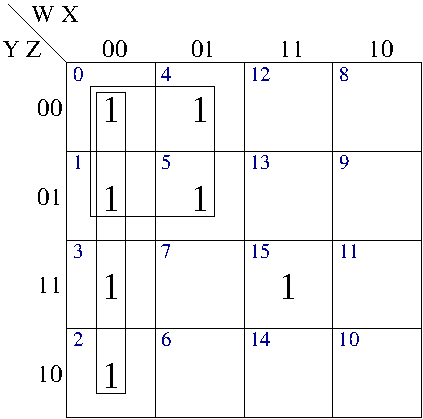
\includegraphics{../CombinationalCircuits/Assessments/4VariableKMapExam}\\ \\
\end{minipage}\\
\medskip
%file: ../CombinationalCircuits/Assessments/circuit_design_ex.tex
10.&\begin{minipage}[t]{\linewidth}(6 pt) Design a digital logic circuit that accepts an unsigned three bit binary number as input and outputs a 1 if that number is either even or a power of 2.  Otherwise, the circuit outputs a 0.  Write a minimal sum of products representation of the logic function for the circuit.

Solution: \\ \\
$F=\sum_{X,Y,Z}(1,2,4,6)=X' \cdot Y' \cdot Z + Y \cdot Z' + X \cdot Z'$\\
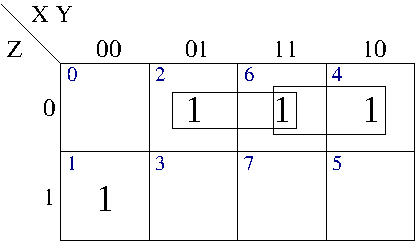
\includegraphics{../CombinationalCircuits/Assessments/CircuitDesignKMapExam}\\
\end{minipage}\\
\medskip
\end{longtable}
\end{document}
